\RequirePackage{filecontents}
\begin{filecontents}{\jobname.bib}
@article{baldini2017,
  author    = {Ioana Baldini and
               Paul C. Castro and
               Kerry Shih{-}Ping Chang and
               Perry Cheng and
               Stephen J. Fink and
               Vatche Ishakian and
               Nick Mitchell and
               Vinod Muthusamy and
               Rodric M. Rabbah and
               Aleksander Slominski and
               Philippe Suter},
  title     = {Serverless Computing: Current Trends and Open Problems},
  journal   = {CoRR},
  volume    = {abs/1706.03178},
  year      = {2017},
  url       = {http://arxiv.org/abs/1706.03178},
  eprinttype = {arXiv},
  eprint    = {1706.03178},
  timestamp = {Mon, 13 Aug 2018 16:47:26 +0200},
  biburl    = {https://dblp.org/rec/journals/corr/BaldiniCCCFIMMR17.bib},
  bibsource = {dblp computer science bibliography, https://dblp.org}
}

@article{rajkumar2017,
  author    = {Rajkumar Buyya and
               Satish Narayana Srirama and
               Giuliano Casale and
               Rodrigo N. Calheiros and
               Yogesh Simmhan and
               Blesson Varghese and
               Erol Gelenbe and
               Bahman Javadi and
               Luis Miguel Vaquero and
               Marco A. S. Netto and
               Adel Nadjaran Toosi and
               Maria Alejandra Rodriguez and
               Ignacio Mart{\'{\i}}n Llorente and
               Sabrina De Capitani di Vimercati and
               Pierangela Samarati and
               Dejan S. Milojicic and
               Carlos A. Varela and
               Rami Bahsoon and
               Marcos Dias de Assun{\c{c}}{\~{a}}o and
               Omer F. Rana and
               Wanlei Zhou and
               Hai Jin and
               Wolfgang Gentzsch and
               Albert Y. Zomaya and
               Haiying Shen},
  title     = {A Manifesto for Future Generation Cloud Computing: Research Directions
               for the Next Decade},
  journal   = {CoRR},
  volume    = {abs/1711.09123},
  year      = {2017},
  url       = {http://arxiv.org/abs/1711.09123},
  eprinttype = {arXiv},
  eprint    = {1711.09123},
  timestamp = {Fri, 22 Apr 2022 11:03:33 +0200},
  biburl    = {https://dblp.org/rec/journals/corr/abs-1711-09123.bib},
  bibsource = {dblp computer science bibliography, https://dblp.org}
}

@article{paul2019,
  author    = {Paul C. Castro and
               Vatche Ishakian and
               Vinod Muthusamy and
               Aleksander Slominski},
  title     = {The server is dead, long live the server: Rise of Serverless Computing,
               Overview of Current State and Future Trends in Research and Industry},
  journal   = {CoRR},
  volume    = {abs/1906.02888},
  year      = {2019},
  url       = {http://arxiv.org/abs/1906.02888},
  eprinttype = {arXiv},
  eprint    = {1906.02888},
  timestamp = {Wed, 04 Dec 2019 15:23:27 +0100},
  biburl    = {https://dblp.org/rec/journals/corr/abs-1906-02888.bib},
  bibsource = {dblp computer science bibliography, https://dblp.org}
}

@article{hassan2017,
author = {Hassan, Hassan and Barakat, Saman and Sarhan, Qusay},
year = {2021},
month = {07},
pages = {},
title = {Survey on serverless computing},
volume = {10},
journal = {Journal of Cloud Computing},
doi = {10.1186/s13677-021-00253-7}
}

@article{jonas2019,
  author    = {Eric Jonas and
               Johann Schleier{-}Smith and
               Vikram Sreekanti and
               Chia{-}che Tsai and
               Anurag Khandelwal and
               Qifan Pu and
               Vaishaal Shankar and
               Jo{\~{a}}o Carreira and
               Karl Krauth and
               Neeraja Jayant Yadwadkar and
               Joseph E. Gonzalez and
               Raluca Ada Popa and
               Ion Stoica and
               David A. Patterson},
  title     = {Cloud Programming Simplified: {A} Berkeley View on Serverless Computing},
  journal   = {CoRR},
  volume    = {abs/1902.03383},
  year      = {2019},
  url       = {http://arxiv.org/abs/1902.03383},
  eprinttype = {arXiv},
  eprint    = {1902.03383},
  timestamp = {Mon, 31 Jan 2022 16:34:15 +0100},
  biburl    = {https://dblp.org/rec/journals/corr/abs-1902-03383.bib},
  bibsource = {dblp computer science bibliography, https://dblp.org}
}

@INPROCEEDINGS{megargel2021,  author={Megargel, Alan and Poskitt, Christopher M. and Shankararaman, Venky},  booktitle={2021 IEEE 25th International Enterprise Distributed Object Computing Conference (EDOC)},   title={Microservices Orchestration vs. Choreography: A Decision Framework},   year={2021},  volume={},  number={},  pages={134-141},  doi={10.1109/EDOC52215.2021.00024}}
\end{filecontents}
\documentclass[a4paper,12pt]{report}
\usepackage[a4paper,inner = 0.5cm, outer = 0.5cm, top = 2cm, bottom = 2cm]{geometry}
\usepackage{filecontents}
\usepackage[english,romanian]{babel}
\usepackage{blindtext}
\usepackage{fancyhdr}
\usepackage{wrapfig}
\usepackage{graphicx}
\usepackage{amsmath}
\usepackage{caption}
\usepackage{dirtytalk}
\usepackage{url}
\usepackage{listings}
\lstset{
basicstyle=\small\ttfamily,
columns=flexible,
breaklines=true
}
\usepackage{fancyvrb}

\renewenvironment{abstract}[1]
  {\bigskip\selectlanguage{#1}%
   \begin{center}\bfseries\abstractname\end{center}}
  {\par\bigskip}

\newcommand{\source}[1]{\caption*{Sursă: {#1}} }

\fancyhf{}
\renewcommand{\headrulewidth}{2pt}
\renewcommand{\footrulewidth}{1pt}
\fancyhead[LE]{\leftmark}
\fancyhead[RO]{\rightmark}
\linespread{1.25}
\hyphenpenalty=50000
\begin{document}
\begin{titlepage}
    \begin{center}
        \begin{figure}[htbp]
            \centering
            \begin{minipage}{0.2\textwidth}
              
\includegraphics[width=\linewidth]{images/poza_stanga.png}
            \end{minipage}\
            \begin{minipage}{0.5\textwidth}
                \begin{large}
                    \textbf{UNIVERSITATEA DIN BUCUREȘTI}\\
                    \\
                    \begin{center}
                    \textbf{FACULTATEA\\
                                DE\\
                    MATEMATICĂ ȘI INFORMATICĂ}
								\end{center}
                \end{large}
            \end{minipage}
            \begin{minipage}{0.2\textwidth}
              
\includegraphics[width=\linewidth]{images/poza_dreapta.png}
            \end{minipage}
        \end{figure}
        
        \vspace*{1cm}
        
        \begin{large}
            \textbf{SPECIALIZAREA INFORMATICĂ}
        \end{large}

        \vspace{2.5cm}
        \begin{LARGE}
            \textbf{LUCRARE DE DISERTAŢIE}\\
            \vspace*{0.5cm}
            \textbf{EXECUŢIA WORKFLOW-URILOR DURABILE ÎN CLOUD}
        \end{LARGE}
            
        \vspace{2.5cm}
        \begin{large}
            \textbf{Absolvent}\\
            \vspace*{0.25cm}
            \textbf{Moldovan George-Alexandru}
        \end{large}
        
        \vspace{2cm}
        \begin{large}
            \textbf{Coordonator științific}\\
            \vspace*{0.25cm}
            \textbf{Lect. dr. Letiţia Marin}
        \end{large}
        
        \vspace{2.5cm}
        \begin{large}
            \textbf{București, septembrie 2022}
        \end{large}
    \end{center}
\end{titlepage}
\newgeometry{a4paper,inner = 1.7cm, outer = 2.7cm, top = 2cm, bottom = 2cm, bindingoffset = 1.2cm}
\begin{abstract}{romanian}
\par Considerând trend-ul ascendent al arhitecturii orientate spre microservicii şi migrarea de la vechiul mod de dezvoltare monolit, această lucrare de disertaţie propune analiza soluţiilor prezente în piaţa în ceea ce priveşte managementul unei arhitecturi pe microservicii în cloud, precum şi analiza unor contribuţii personale aduse unui framework open-source de gestionare a workflow-urilor în cloud. Sistemele informatice preiau din complexitatea operaţiilor de zi cu zi, astfel că arborii de decizie trebuie interpretaţi şi gestionaţi în mod corect pentru a realiza un sistem care să indeplinească cerinţele de piaţă curente. Pentru o lungă perioadă de timp, problema gestionării tranzacţiilor distribuite si management-ul workflow-urilor a fost inexistentă, deoarece într-un sistem monolit, caracteristicile tranzacţionale ale bazelor de date ce susţineau astfel de sisteme erau îndeajuns pentru a avea toate garanţiile necesare astfel încât sistemul să fie mereu lăsat într-o stare consistentă. În cazul microserviciilor şi arhitecturilor distribuite in general, deşi vin cu o serie lungă de avantaje, poate cel mai greu de gestionat lucru este management-ul stării unei acţiuni, atunci când aceasta se întinde pe mai multe microservicii, şi pe o durată lungă de timp. 
\end{abstract}
\begin{abstract}{english}\par Considering the upward trend of microservices-oriented architecture and the migration from the old monolithic development mode, this dissertation aims to analyze the solutions present in the market in terms of managing a microservices architecture in the cloud, and the analysis of personal contributions to a open-source framework for managing cloud workflows. Information systems take over the complexity of day-to-day operations, so decision trees must be interpreted and managed correctly to achieve a system that meets current market requirements. For a long time, the problem of distributed transaction management and workflow management was non-existent, because in a monolithic system, the transactional characteristics of the databases that supported such systems were sufficient to have all the necessary guarantees so that the system should always be left in a consistent state. Distributed microservices and architectures in general, although they come with a long list of advantages, perhaps the most difficult thing to manage is the management of the state of an action, when it extends over several microservices, and over a long period of time.
\end{abstract}
\tableofcontents
\pagenumbering{arabic}
\setcounter{page}{2}
\chapter{Introducere}
\section{Motivaţie}
\quad Unul din principiile de bază ale programării este reutilizarea. Motivaţia din spatele acestei lucrări o reprezintă dorinţa de a contribui la un framework care rezolvă o problemă generică, cu care se confruntă toţi dezvoltatorii care trebuie să gestioneze tranzacţii distribuite. Analiza diferitelor metode pentru rezolvarea problemei de gestiune a workflow-urilor în cloud, în special într-o arhitectură ce se bazează pe funcţii în cloud, a fost o prioritate pentru mine în ultimii ani. 
\par
Serverless, sau Functions-as-a-Service (FaaS), este o paradigmă din ce în ce mai populară pentru dezvoltarea de aplicații, deoarece oferă scalare infinită implicită și facturare bazată pe consum. Cu toate acestea, garanţiile slabe de execuţie și suportul nativ pentru stocare a stării a FaaS creează provocări serioase atunci când se dezvoltă aplicații care necesită stare persistentă, garanţii de execuţie sau sincronizare. Acest lucru a motivat o nouă generație de soluţii serverless care oferă abstractizări ce stochează starea aplicaţiei. Un exemplu în acest sens, noua soluţie Azure Durable Functions (DF), o extindere peste deja existenta Azure Functions. Modelul îmbunătățește FaaS cu actori, fluxuri de lucru și secțiuni critice.
\par
În acest context în care dezvoltatorii încearcă să dezvolte aplicaţii ce gestionează workflow-uri  de lungă durată, cu toţii rezolvă aceeaşi problemă şi anume lipsa separării între nivelul de execuţie şi nivelul de stocare a soluţiilor existente FaaS. Cu toţii rezolvă o problemă generică, de salvare a stării în anumite puncte ale execuţiei, pentru a putea relua workflow-ul în eventualitatea în care agentul pe care rulează aplicaţia pică inainte de finalizarea workflow-ului. Acest lucru era foarte greu de realizat în arhitecturi serverless deoarece toate soluţiile existente până la apariţia Azure Durable Functions, suportau doar execuţii stateless în mod standard. Deci până la apariţia soluţiilor ce oferă garanţii de execuţie puternice în lumea Serverless, această tehnologie nu era o opţiune populară pentru dezvoltarea aplicaţiilor ce aveau nevoie de gestionare a stării şi era limitată la execuţia unor părţi mici ale aplicaţiilor pentru care stările intermediare nu erau importante. 
\section{Context}
\quad Serverless diferă de conceptele tradiționale de cloud computing în sensul că infrastructura și platformele în care serviciile rulează sunt ascunse clienților. În această abordare, clienții sunt preocupați doar de funcționalitatea dorită a aplicației lor, iar restul este delegat furnizorului de servicii. \par

Scopul serviciilor Serverless este triplu : 
\begin{itemize}
\item Scuteşte dezvoltatorii de servicii cloud de la interacţiunea cu infrastructura sau diferite platforme;
\item Converteşte modelul de facturare din cel clasic la cel bazat pe consum;
\item Permite scalarea automată a serviciului în funcție de cererea clienților.
\end{itemize}
\par

\begin{wrapfigure}{r}{0.45\textwidth}
	  \begin{center}
        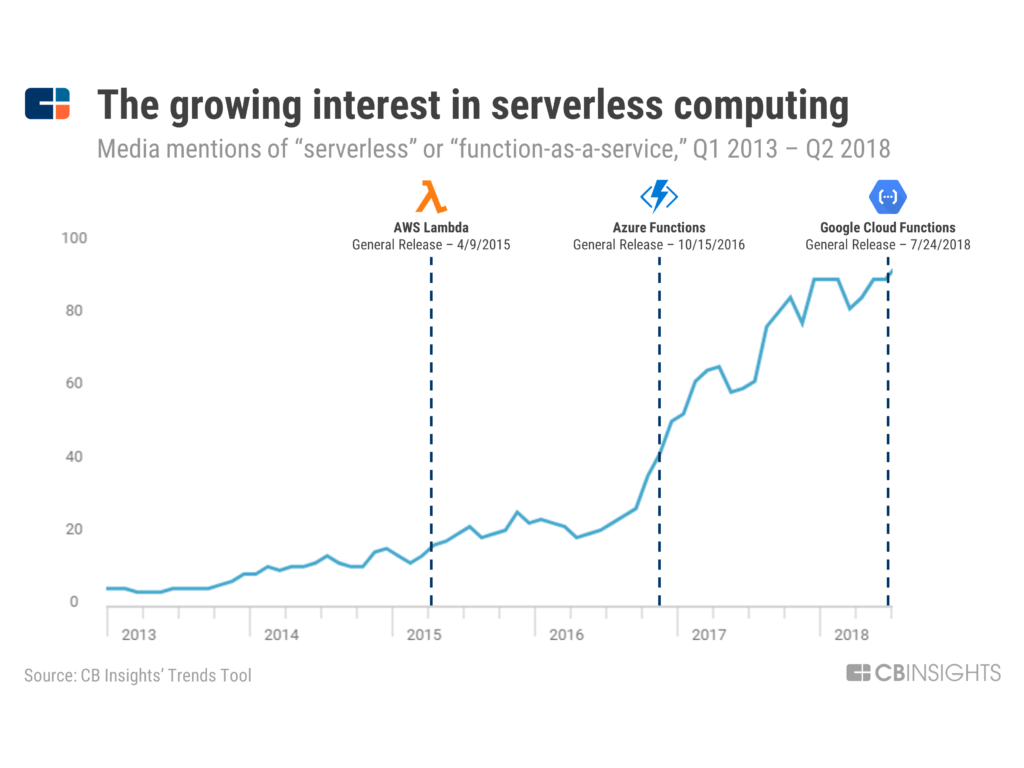
\includegraphics[width=0.4\textwidth]{images/grafic_serverless_computing}
       \caption{Statistică ce evidenţiază importanţa domeniului cloud computing în ultimii ani}
			\label{fig:cloud_computing_graph}
       \source {https://www.cbinsights.com}
    \end{center}
\end{wrapfigure}
Ca rezultat, într-o aplicație cu adevărat Serverless, infrastructura de execuție este ascunsă clientului, iar clientul plătește doar pentru resursele pe care le utilizează efectiv. Serviciul este conceput astfel încât să poată gestiona rapid creșterile de consum prin scalare automată. Entitățile de bază în calculul fără server sunt funcții. Clientul își înregistrează funcțiile în furnizorul de servicii. Apoi, acele funcții pot fi invocate fie de un eveniment, fie direct prin apelarea acestora la cererea utilizatorilor. Rezultatele execuției sunt trimise înapoi clientului. Invocarea funcțiilor este delegată unuia dintre nodurile de calcul disponibile în interiorul furnizorului de servicii.

\par
Deși conceptul de Serverless este relativ nou, acesta și-a deschis drumul în multe aplicații din lumea reală, de la instrumente de colaborare online la sisteme integrate (IoT), având o creştere în adopţie foarte rapidă, lucru vizibil şi în figura ~\ref{fig:cloud_computing_graph}. Această creştere este datorată în mare parte usurinţei procesului de dezvoltare a aplicaţiilor Serverless şi beneficiilor pe care le aduc din punct de vedere al scalării în mod automat, şi al gestionării complete a infrastructurii ce stă la baza aplicaţiilor. 
\par
Unul din lucrurile care poate duce adopţia tehnologiei serverless la un cu totul alt nivel, este tocmai capacitatea de a putea dezvolta aplicaţii întregi, ce se pot baza pe starea sistemului în cadrul execuţiei, precum şi capacitatea de a gestiona long running workflows, o nevoie care este prezentă în mai toate aplicaţiile curente. 
\section{Alte analize ale problemelor curente a arhitecturii Serverless}
\quad Există mai multe provocări cu care se confruntă în prezent serviciile Serverless. Există unele sondaje și recenzii ale literaturii care discută aceste provocări \cite{baldini2017,rajkumar2017,paul2019,hassan2017,jonas2019}.
\par\emph{Baldini et al.} \cite{baldini2017} enumeră o serie de probleme cu care se confruntă arhitectura serverless, printre care costul, care reprezintă un avantaj pentru această arhitectură doar dacă se execută metode care nu sunt bazate pe prelucrare input-output. Altfel, este mai eficient din punct de vedere al costurilor folosirea soluţiilor clasice în cloud cum ar fi maşini virtuale rezervate sau containere. O altă problemă semnalată este cea a cold-start-ului care poate face o aplicaţie bazată pe funcţii serverless să pară înceată dacă pentru fiecare apel este necesar un cold start, din cauză că traficul nu este indeajuns de mult pentru a împiedica funcţia să scaleze la 0. 
\par\emph{Rajkumar et al.} \cite{rajkumar2017} discută despre dificultăţile dezvoltării unei arhitecturi serverless din punct de vedere al limitărilor cu care vine această nouă tehnologie şi anume limitările de timp al execuţiei, de memorie a agentului şi de management al stării. Acesta crede că este nevoie de o schimbare a mentalităţii de dezvoltare a aplicaţiilor pentru a beneficia la adevaratul potenţial al tehnologiilor Serverless, iar momentul în care aplicaţiile enterprise complete vor fi migrate sau dezvoltate complet pe o arhitectură Serverless este încă departe. Autorul vede această tehnologie ca pe o unealtă ajutătoare în dezvoltarea aplicaţiilor, dar pe viitor poate ajunge să fie nucleul aplicaţiilor.  
\par\emph{Castro et al.} \cite{paul2019} ridică problema dezvoltării de aplicaţii stateful folosind tehnologii Serverless în viitor, o temă ce în acea perioadă era doar o idee, dar după cum urmează sa fie prezentat în această lucrare, acum este o realitate. Alte probleme menţionate ar fi usurinţa cu care poate fi portată o aplicaţie legacy către o arhitectură Serverless, deoarece nu este de dorit sa se piardă toate acele ore valoroase care au fost deja investite în aplicaţiile existente. 
\par\emph{Hassan et al.} \cite{hassan2017} discută despre problema limitării la un singur provider atunci cand vine vorba de arhitecturi serverless, deoarece codul pentru un anumit provider de exemplu AWS Lambda, nu e portabil către alt provider, de exemplu Microsoft Azure Functions. 
\par\emph{Jonas et al.} \cite{jonas2019} prezintă ineficienţele arhitecturii serverless atunci când vine vorba de procesarea operaţiilor care în mod normal ar beneficia de pe urma unui sistem cu mai multe nuclee şi implicaţiile pe care aceasta limitare (2 nuclee per funcţie) o are atunci când vine vorba de paralelizarea acţiunilor pentru a îmbunătăţi viteza. Impactul major în acest caz este creşterea semnificativă a datelor transmise pe reţea pentru a obţine acelaşi grad de paralelism într-un sistem serverless versus unul clasic în cloud. 


\section{Conţinutul lucrării}
 Din punct de vedere al structurii, lucrarea va fi organizată în 2 părţi :
\begin{itemize}
\item Partea teoretică în care va fi analizat Durable Task Framework şi modul în care funcţionează acesta;
\item Partea practică ce va compara aceeaşi aplicaţie, dezvoltată în 2 moduri (clasic şi folosind DTF).
\end{itemize}
\par În prima parte a lucrării va fi analizată tehnologia ce stă la baza soluţiilor de management al workflow-uri în cloud si anume, Durable Task Framework. Vom analiza modul în care este separat domeniul de execuţie de domeniul de stocare, care sunt interfeţele pe care trebuie să le respecte un provider, care sunt constrângerile care trebuie respectate atunci când se foloseşte această tehnologie şi, bineînţeles, care sunt beneficiile şi dezavantajele sale. 
\par În a 2-a parte va fi analizat un exemplu clasic în literatura managementului de workflow-uri şi anume cazul de rezervare multiplă în cazul unei călatorii. Această mini-aplicaţie a fost dezvoltată atât folosind metode clasice, cât şi folosind Durable Task Framework. Folosind aceste 2 abordări, vor fi analizate : 
\begin{itemize}
\item Capacităţile fiecărui sistem şi nivelul de rezilienţă împotriva dezastrelor pe care îl pot demonstra;
\item Diferenţele de dezvoltare între cele 2 abordări;
\item Analiză teoretică a costurilor între cele 2 arhitecturi; 
\item Performanţa celor 2 sisteme.
\end{itemize}
\chapter{Analiza Tehnologiei Durable Task Framework }
\section{Analiză generală}
\quad Durable Task Framework (DTFx) este o bibliotecă care permite utilizatorilor să gestioneze workflow-uri persistente de lungă durată (denumite orchestrări) în C\# folosind sintagme clasice de codare async/await. DTF stă la baza soluţiilor Microsoft de gestionare a workflow-urilor durabile în cloud . Folosind această tehnologie, a fost expusă prima soluţie serverless ce permite gestionarea stării : Azure Durable Functions. 
\par Din punct de vedere al arhitecturii framework-ului, acesta are 2 părţi:
\begin{itemize} 
\item DTF Core, ce conţine nivelul de abstractizare al gestionării, şi implementează conceptele de bază ce permit programarea orchestrărilor folosind sintagme async await;
\item DTF providers, care implementează interfeţele expuse de Core pentru a folosi diferite medii de stocare, în funcţie de nevoile dezvoltatorului. 
\end{itemize} 
\par La bază, framework-ul îşi propune să rezolve problema durabilităţii acţiunilor într-un sistem distribuit, în care este de aşteptat ca orice piesă a sistemului poate pica în orice moment. Arhitectura framework-ului e bazată pe evenimente, spre deosebire de alte framework-uri anterioare ce se bazau pe stocarea întregii stări a aplicaţiei la un moment dat. 
\par Nevoia de garanţii de execuţie a făcut ca DTF să construiască un sistem ce permite construcţia unei structuri arborescente ce reprezintă o maşină de stări finite, în care, frunzele arborelui (activităţile, în terminologia DTF) au garanţia că vor fi executate cel puţin o dată. Această garanţie vine şi cu o constrângere : din cauză că activităţile nu sunt executate \textbf{exact o dată} este necesar ca toate acţiunile din cadrul unei activităţi sa fie idempotente. 
\section{Folosirea evenimentelor în DTF}
\quad Modelul de arhitectură bazat pe evenimente este un model popular de arhitectură asincronă distribuită, utilizat pentru a produce aplicații foarte scalabile. De asemenea, este foarte adaptabil și poate fi utilizat pentru aplicații mici și, de asemenea, pentru cele mari și complexe. Arhitectura bazată pe evenimente este alcătuită din componente de procesare a evenimentelor extrem de decuplate, cu un singur scop, care primesc și procesează evenimentele în mod asincron.

Modelul de arhitectură bazat pe evenimente constă din două topologii principale, mediatorul și brokerul. Topologia mediatorului este folosită în mod obișnuit atunci când există nevoia de orchestrare a mai multor pași în cadrul unui eveniment printr-un mediator central, în timp ce topologia brokerului este utilizată atunci când dorim să înlănțuim evenimente fără a utiliza un mediator central. Deoarece caracteristicile arhitecturii și strategiile de implementare diferă între aceste două topologii, este important ca ambele să fie cunoscute pentru a putea întelege motivaţia din spatele alegerii arhitecturii DTF. 

\par Gestionarea workflow-urilor prin mediator central, cunoscută şi drept \textbf{Orchestrare} în literatura de specialiate (\emph{Megargel et al.}\cite{megargel2021}), constă în prezenţa unei entităţi centrale ce comunică cu toate celelalte sisteme ce iau parte la un anume workflow pentru a garanta execuţia cu success a unei maşini de stări. Topologia mediatorului este utilă pentru evenimentele care au mai mulți pași și necesită un anumit nivel de orchestrare pentru a procesa evenimentul. Aşa cum vom vedea şi în partea practică a acestei lucrări, sunt nenumărate cazuri ce se reduc la gestionarea unei maşini de stări. Un astfel de exemplu este un lanţ de aprovizionare, în care, de la momentul achiziţiei până la momentul livrării sunt numeroase etape ce trebuie îndeplinite cu success pentru ca operaţiunea ca un întreg sa fie un succes. Printre acest etape, s-ar număra pregătirea coletului, predarea lui către firma de curierat, înregistrarea plăţii şi în final, livrarea propriu zisă. Un astfel de sistem poate beneficia de un mediator central, care asigură gestiunea stării unui astfel de workflow. 
\par Gestionarea workflow-urilor printr-o topologie cu broker, cunoscută drept  \textbf{Coreografie}, constă în distribuirea gestiunii maşinii de stări între toţi consumatorii evenimentelor, astfel încât fiecare poate lua o anumită decizie în funcţie de contextul în care se află atunci când procesează un eveniment. În această topologie nu există un mediator central, iar fiecare participant în workflow are responsabilitatea deciderii următoarei acţiuni, în momentul procesării unui eveniment. Astfel, acest gen de arhitectură este potrivită pentru worfklow-uri minimale, fără maşini de stări complicate, care nu au nevoie de un loc centralizat pentru asigurarea consistenţei stării. Altfel, folosind această arhitectură în sisteme complexe, se poate ajunge foarte repede la haos, deoarece deciziile sunt împărţite peste tot, devenind imposibilă urmărirea firului logic al unei astfel de execuţii distribuite. 
\begin{figure}[h]
\begin{center}
        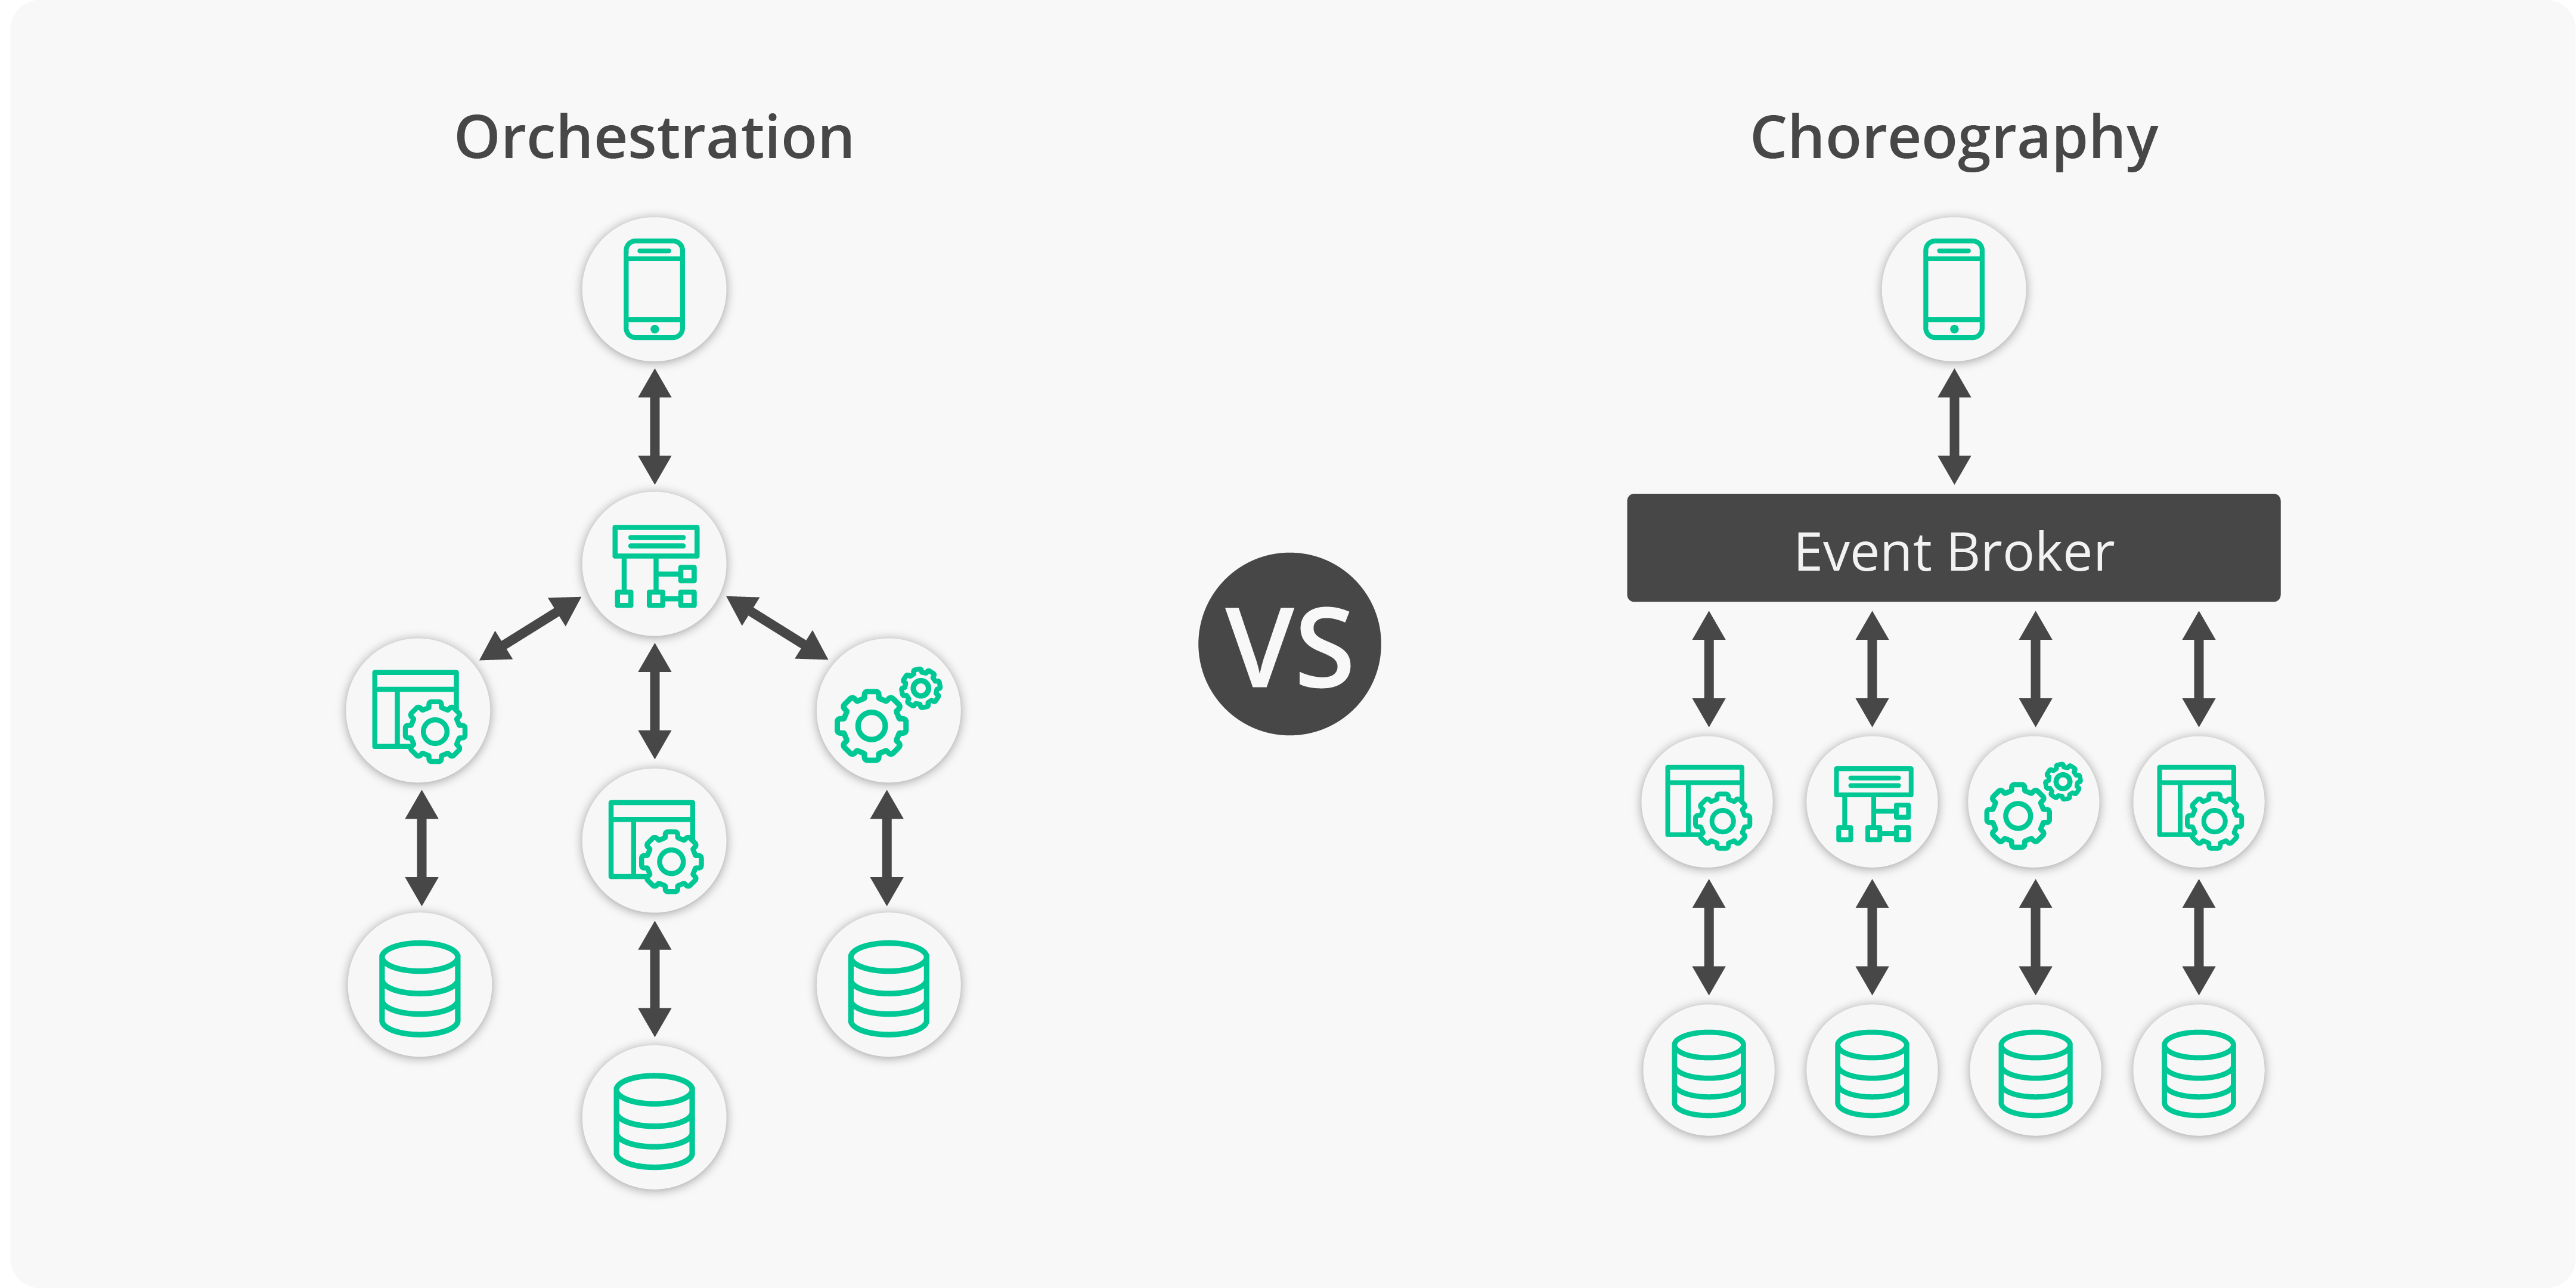
\includegraphics[width=1\textwidth]{images/Orchestration-VS-Choreography}
			 \caption{Orchestrare versus Coreografie}
			 \label{fig:orch_vs_coreografie}
			 \source {https://solace.com/blog/microservices-choreography-vs-orchestration/}
\end{center}
\end{figure}

\par Durable task framework, implementează o arhitectură de tip mediator central, si expune bazele pentru a putea crea propriul mediator pentru gestiunea unui workflow de lungă durată. Pentru a analiza implementarea conceptului de orchestrare bazată pe evenimente, vom analiza implementarea de DTF împreună cu Sql Server Provider, pentru a face o transpunere a conceptelor teoretice în lumea DTF. În figura ~\ref{fig:sql-server-provider} se poate observa structura schemei ce susţine framework-ul atunci cand este rulat împreuna cu un SQL Server Provider. Acesta implementează conceptele teoretice într-un nivel de stocare bazat pe SQL server. 
 
 \begin{figure}[h]
\begin{center}
        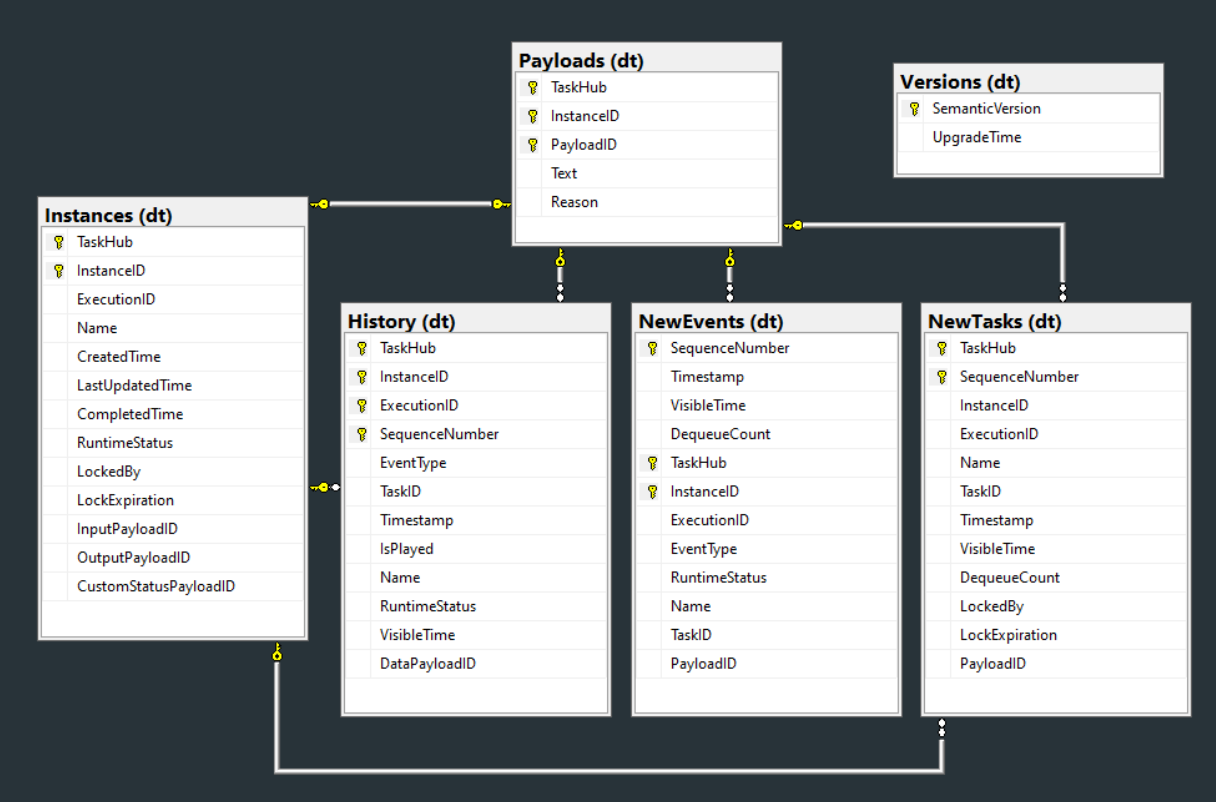
\includegraphics[width=1\textwidth]{images/sql-server-provider}
			 \caption{DTF Schema în DTF Sql Server provider}
			 \label{fig:sql-server-provider}
			 \source {https://microsoft.github.io/durabletask-mssql/}
\end{center}
\end{figure}

\par Există patru tipuri principale de componente de arhitectură în topologia mediatorului: 
\begin{itemize}
\item cozi de evenimente
\item mediatorul de evenimente
\item canale de evenimente
\item procesatoarele de evenimente. 
\end{itemize}
\par Fluxul de evenimente începe cu un client care trimite un eveniment la o coadă de evenimente, care este utilizată pentru a transporta evenimentul la mediatorul de evenimente. Mediatorul de evenimente primește evenimentul inițial și orchestrează acel eveniment prin trimiterea de evenimente asincrone suplimentare către canalele de evenimente pentru a executa fiecare pas al procesului. Procesatoarele de evenimente, care ascultă pe canalele de evenimente, primesc evenimentul de la mediatorul de evenimente și execută o logică de afaceri specifică pentru a procesa evenimentul.  Vom analiza fiecare componentă teoretică a procesului pentru a stabili parelela către structura din DTF, urmărind schema prezentată în figura ~\ref{fig:sql-server-provider}.
\par În cazul nostru, coada de eveniment este tabela `New Events` iar modalitatea prin care un eveniment ajunge în aceasta, este prin folosirea unui DTF Client pentru a inregistra un eveniment pentru o anumita orchestrare. 
\par Mediatorul de evenimente este `Orchestrarea` respectiv logica definită de dezvoltator pentru a gestiona workflow-ul. Această logică este rulată de fiecare dată când un eveniment este primit pentru un anume workflow. Deşi codul este rulat de mai multe ori, operaţiune denumita şi `Replay`, acţiunile care deja au mai fost executate o dată nu sunt re-executate, ci rezultatele lor sunt direct încărcate direct din memorie, folosind istoricul orchestrării. Istoricul este salvat in tabela `History`.
\par Canalele de evenimente sunt diferitele Task-uri înregistrate în tabelul `NewTasks`. Acestea sunt folosite de pentru a declanşa execuţia unor Activităţi, ce reprezintă frunzele arborelui de execuţie a unui workflow. Task-urile sunt înregistrate pe canalele de evenimente de catre mediatorul de evenimente, pentru a fi mai apoi procesate de procesatorul de evenimente. La finalul procesării unui task din canalul de evenimente, procesatorul de evenimente emite un nou eveniment pe coada de evenimente, pentru ca mediatorul să poate continua execuţia workflow-ului. 
\par Procesatoarele de evenimente sunt Workerii de DTF şi reprezintă logica din DTF Core care monitorizează în mod constant canalele de evenimente pentru a prelua eventualele noi Task-uri ce sunt disponibile pentru execuţie. Astfel, se obţine o arhitectură foarte decuplată în care inregistrarea de evenimente, gestionarea stării workflow-ului, execuţia propriu zisă a diverselor task-uri şi întoarcerea răspunsurilor înapoi către mediator sunt toate operaţiuni decuplate, independente una de cealaltă.
\par Cel mai important aspect ce reiese din analiza implementării conceptelor de orchestrare bazată pe evenimente, este că datorită operaţiilor independente, eşecurile care pot apărea atunci când această logica este executată într-un mediu distribuit nu vor afecta starea workflow-ului ca un întreg, fiindcă eşecul într-o parte a arhitecturii nu afectează alte părţi, iar fiecare unitate este independent reîncercabilă. Astfel, revenirea în urma unui eşec (eroare de reţea, deconectare completă fie a workerilor fie a client-ului) sunt gestionate într-un mod elegant, fără efecte secundare. 

\section{DTF în Durable Functions} 
\quad Conceptele prezentate în capitolul anterior, au fost reimplementate in DTF pentru a putea executa această tehnologie folosind soluţii native în cloud, şi pentru a expune o soluţie pentru care există o mare nevoie în piaţă : Statefull Serverless functions. Astfel, a fost dezvoltat un nou provider pentru DTF, bazat pe Azure Storage tables de această dată, pentru a expune aceeaşi functionalitate şi în cloud. 
\par Logica de bază a framework-ului a ramas aceeaşi, în schimb implementarea celor 4 concepte de bază într-o arhitectură bazată pe evenimente (cozi de evenimente, mediatorul de evenimente ,canale de evenimente, procesatoarele de evenimente) este schimbată.
\par Această adaptare a dus la lansarea unei soluţii noi pe piaţă ce a creat un cu totul nou domeniu în lumea serverless: funcţii ce sunt capabile ce gestioneze starea, si să ruleze o perioada foarte îndelungată de timp, dar pentru care se plăteşte doar timpul de execuţie propriu zis. Acest lucru vine cu beneficii foarte mari din punct de vedere al costurilor, deoarece într-un workflow ce conţine şi paşi manuali, cum ar fi aprobarea de către un operator a unei trazacţii, pe perioada în care se aşteaptă acest eveniment, codul orchestrării nu se execută, deci practic nu există un cost asociat acestei operaţii. 
\par Pe lângă functionalităţile ce există în mod standard în toţi providerii de DTF, Durable Functions vine cu o caracteristică suplimentară numită Durable Entities. Durable Entities definesc operațiuni pentru citirea și actualizarea unor mici părți de stare, cunoscute sub numele de entități durabile. La fel ca funcțiile de orchestrator, funcțiile de entitate sunt funcții cu un tip de declanșator special, declanșatorul de entitate. Spre deosebire de funcțiile de orchestrator, funcțiile de entitate gestionează starea unei entități în mod explicit, mai degrabă decât să reprezinte implicit starea prin fluxul de control. Entitățile oferă un mijloc de extindere a aplicațiilor prin distribuirea lucrării în mai multe entități, fiecare cu o stare de dimensiuni modeste. Practic, acest lucru oferă suport automat pentru gestiunea unei stări independente de cea a orchestrării, dar într-un mod distribuit şi sigur, deoarece oferă garanţii de access serializat la aceasta. 
 \begin{figure}[h]
\begin{center}
        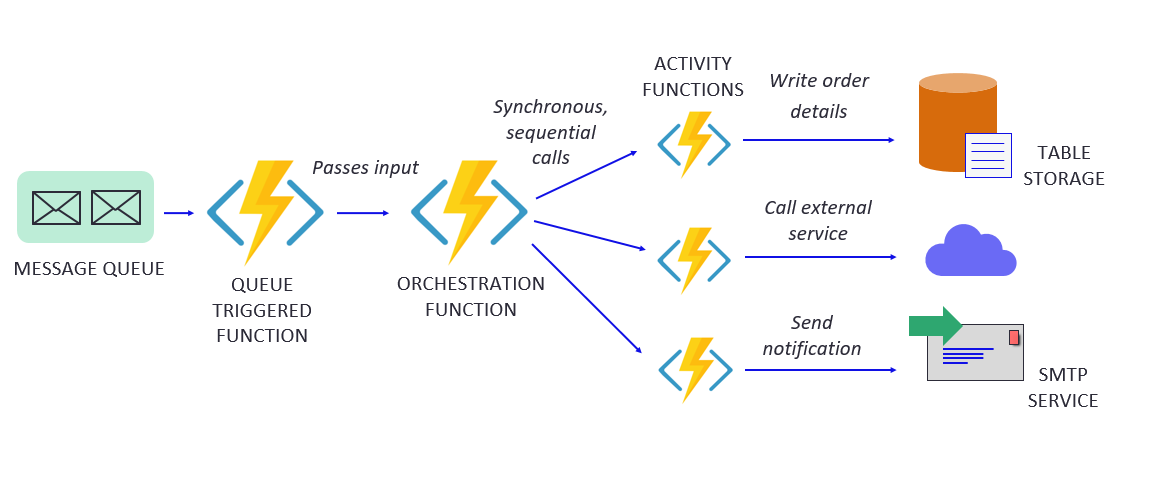
\includegraphics[width=1\textwidth]{images/durable-functions}
			 \caption{Exemplu arhitectură folosind Durable Functions}
			 \label{fig:durable-functions}
			 \source {https://thisiszone.medium.com}
\end{center}
\end{figure}
\par Aşa cum se poate observa şi în figura ~\ref{fig:durable-functions}, conceptele clasice de DTF sunt transpuse în funcţii individuale, de diferite tipuri. Astfel, o orchestrare este reprezentată de un Orchestration Function, o activitate este reprezentată de un Activity Function, în timp ce starea globală a workflow-ului este stocată în tabele în Azure Storage. Obţinem astfel o arhitectură nativă în cloud, fară costuri de mentenanţă a infrastructurii şi de scalare, având ca beneficiu principal faptul că gestionarea stării într-un mediu distribuit nu mai este responsabilitatea explicită a dezvoltatorului, ci este rezolvată implicit de către providerul de soluţii cloud. 
\section {Dificultăţi în gestionarea workflow-urilor de lungă durată - Versionarea Orchestrărilor }
\quad Pe langă beneficiile pe care le are o arhitectură bazată pe un mediator pentru gestiunea workflow-urilor, această centralizare are şi anumite limitări si dezavantaje. Printre aceastea, poate cel mai dificil lucru de gestionat este versionarea acestora.
\par Natura îndelungată a acestor workflow-uri face ca acestea să aibă următoarele particularităţi: 
\begin{itemize}
\item Un workflow poate dura mai mult de un ciclu de dezvoltare (Mai multe versiuni ale aceluiaşi workflow pot exista până când o anumită instanţă a unei anume versiuni finalizează execuţia). 
\item Codul de orchestrare trebuie să fie determinist deoarece acesta va fi executat de mai multe ori pe perioada de viaţă a unui workflow. 
\end{itemize}
\par Prima problema se rezumă la dificultatea de versionare a unei orchestrări. Atunci cand va apărea o versiune nouă a maşinii de stări gestionată de o anume orchestrare, cea veche nu poate fi direct înlocuită, deoarece încă există instanţe ale acelui tip de workflow care înca rulează. Astfel, versiunile noi de orchestrare trebuie mereu rulate în paralel cu cele vechi, până când toate instanţele ce rulează versiunea veche a workflow-urilor finalizează execuţia. În acel moment versiunea veche a orchestrării va putea fi ştearsă. 
\par Cea de-a doua problemă este mai mult doar o limitare şi anume, din cauza logicii de replay pe perioada de viaţă a unei orchestrări, dezvoltatorul trebuie sa se asigure ca tot codul sursă din cadrul unei orchestrări va returna acelaşi rezultat indiferent de momentul în care se rulează. Pe scurt, comportamentul unei orchestrări trebuie sa fie determinist şi constant indiferent de timp. 
 \begin{figure}[h]
\begin{center}
        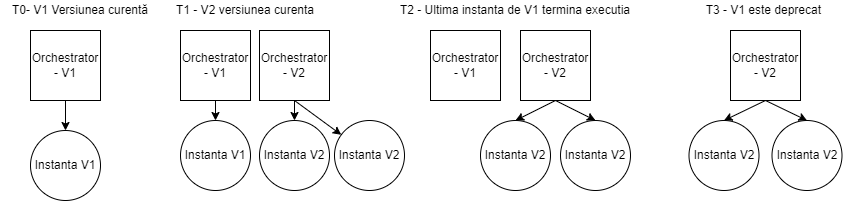
\includegraphics[width=1\textwidth]{images/dtf_versioning}
			 \caption{Ciclu de versionare a codului de orchestrare}
			 \label{fig:dtf-versioning}
\end{center}
\end{figure}
\chapter{Workflow-uri de lungă durată - Analiză paralelă a arhitecturii}
\section{Descrierea problemei}
\quad Atunci când vine vorba de managementul unui workflow de lungă durată, sau a unei tranzacţii distribuite, un exemplu clasic în literatură este cel al unei rezervări de călătorie. O rezervare de călătorie presupune mai multe etape : 
\begin{itemize}
\item Rezervarea unui taxi;
\item Rezervarea hotelului;
\item Rezervarea avionului.
\end{itemize}
\par Într-o lume monolitică, în care totul ar fi deţinut de un singur serviciu ale cărei arhitecturi s-ar fi bazat pe o bază de date relaţională, garantarea rezervării cu success ar fi fost o problemă uşor de rezolvat având în vedere caracteristica de atomicitate a unei tranzacţii. În schimb, într-o lume distribuită, în care fiecare serviciu este complet independent (Taxi Pelicanul, Hotel Capşa şi Blue Air ) sistemul de gestiune a unei rezervări trebuie să fie rezilient la toate erorile ce pot apărea la diferite niveluri ale aplicaţiei. Astfel sistemul nostru trebuie să garanteze nu numai că rezervarea se face cu success, dar în cazul în care acest lucru nu se face, toate sistemele să fie aduse la starea iniţială de dinaintea începerii tranzacţiei distribuite.
\par Recuperarea dintr-un eşec într-o tranzacţie distribuită nu se poate face în mod nativ, deoarece aplicaţiile ce iau parte la aceasta sunt complet independente, astfel că fiecare sistem ce participă la o astfel de tranzacţie trebuie să expună şi o funcţionalitate de roll-back ce va anula o operaţie executată anterior. Astfel, putem concluziona că managementul unei tranzacţii distribuite rezultă întotdeauna în managementul unui workflow de tip SAGA. 
\par Saga este un concept arhitectural teoretic ce garantează execuţia unui workfow într-un mod predictibil: Fie \(A_{1}, A_{2}, .... A_{n}\) acţiuni ce participă la o execuţie Saga şi \(RA_{1}, RA_{2}, .... RA_{n}\) acţiunile de rollback corespunzător fiecărui pas din workflow. Un workflow de tip Saga garantează fie că toţi paşii \(A_{1}, A_{2}, .... A_{n}\) au fost executaţi cu succes, fie \(A_{1}, A_{2}, .... A_{t} , RA_{1}, RA_{2}, ..... RA_{t}\) au fost executaţi cu succes. Astfel, se garantează fie că toate acţiunile au fost executate cu success, fie că toate acţiunile ce au apucat să fie executate până la un punct de eroare au fost anulate cu succes. În final, sistemul va fi mereu într-o stare consistentă. 
\par Scopul părţii practice a acestei lucrări este implementarea unui coordonator de tranzacţii distribuite de lungă durată implementând o arhitectură Saga. Vor fi analizate atât dezvoltarea acestei aplicaţii folosind un framework care facilitează dezvoltarea orchestratoarelor, cât şi dezvoltarea aplicaţiei folosind tehnologii clasice (.net Web API  combinat cu o bază de date relaţională). 
\section{Implementarea arhitecturii în mod clasic}
\par În mod clasic, implementarea unui serviciu ce oferă garanţiile unei arhitecturi SAGA, trebuie să fie rezistent la următoarele potenţiale probleme :
\begin{itemize}
\item Posibilitatea ca procesul să fie închis chiar în timpul execuţiei;
\item Posibilitatea ca unul din paşi să eşueze din motive neimputabile sistemelor ce iau parte la acţiune (probleme de reţea).
\end{itemize}
\subsection{Implementarea naivă}
Vom porni de la următoarea secvenţă de cod : 
\begin{Verbatim}[numbers=left]
var step = ''Started'';
try {
	await sagaService.bookHotel(booking);
	step = ''BookedHotel'';
	await sagaService.bookTaxi(booking);
	step = ''BookedTaxi'';
	await sagaService.bookFlight(booking);
	step = ''BookedFlight'';
} catch (Exception){
	if (step ==  ''BookedHotel''){
		await sagaService.cancelHotel(booking);
	} else if (step ==  ''BookedTaxi''){
		await sagaService.cancelHotel(booking);
		await sagaService.cancelTaxi(booking);
	}
}
\end{Verbatim}
Într-un sistem monolit această secţiune de cod ar fi o implementare corectă a unui SAGA, dar ce se poate întâmpla dacă analizăm cazurile la care trebuie să fie rezilient un astfel de sistem, într-o configuraţie distribuită ? 
\par Analizând prima potenţială problemă şi anume posibilitatea ca procesul ce execută Saga să fie oprit în mijlocul execuţiei, putem evidenţia potenţialele probleme cu această abordare. Practic, daca serverul este oprit oriunde între linia 4 si 14, va lăsa execuţia într-o stare inconsistentă, cu posibilitatea de a avea consecinţe serioase asupra utilizatorului. Ce se întamplă dacă se execută doar rezervarea de Hotel, dar utilizatorul nu este notificat ? Acestuia îi va fi retrasă suma de pe card în mod abuziv, rezultând în posibile probleme legale pentru deţinătorul aplicaţiei. Astfel, garanţia atomicităţii într-o tranzacţie distribuită este foarte importantă. 
\par Motivele pentru care această întrerupere a execuţiei practic face imposibilă garantarea atomicităţii întregii operaţii, este că toată acţiunea se execută ca parte a unei singure încercări, şi orice întrerupere a firului de execuţie face ca operaţia să nu poată fi reîncercată şi eventual continuată, pentru a garanta execuţia completă a strategiei Saga. 
\subsection{Execuţie durabilă}
\par O altă problemă cu codul iniţial este că nu acoperă nici posibilitatea ca unul din paşi să eşueze din motive de probleme de reţea, iar astfel, toată operaţiunea poate rămâne într-o stare inconsistentă, dacă pe perioada roll-back-ului (între linia 10 si 14) unul din paşi eşuează. Pentru a acoperi ambele probleme, codul ar trebui să fie transformat dupa cum urmează : 
\begin{Verbatim}[numbers=left]
var booking = await sagaService.RegisterIfNotPresent(booking); // returneaza starea 
// inregistrata in baza de date a rezervării sau inregistreaza rezervarea 
// în baza de date, daca este prima execuţie.
try {
	if (!booking.isHotelBooked){
		await sagaService.bookHotel(booking);
		await sagaService.saveState(booking);
		}
	if (!booking.isTaxiBooked){
		await sagaService.bookTaxi(booking);
		await sagaService.saveState(booking);
	}
	if (!booking.isFlightBooked){
		await sagaService.bookFlight(booking);
		await sagaService.saveState(booking);
	}
} catch (Exception){
	try{
		if (booking.isHotelBooked){
			await sagaService.cancelHotel();
			await sagaService.saveState(booking);
		} else if (booking.isTaxiBooked){
			await sagaService.cancelHotel();
			await sagaService.cancelTaxi();
			await sagaService.saveState(booking);
		}
	}
	catch (Exception){
		await sagaService.markAsFailed(booking);
	}
}
\end{Verbatim}
Odată cu modificarea secvenţei de cod, putem observa următoarele modificări :
\begin{itemize}
\item Introducerea unui nivel de decuplare, la nivelul bazei de date, ce permite execuţia repetată a secvenţei de cod fără a pierde starea precedentă, pentru a evita trimiterea mai multor request-uri prin reţea decât este necesar; 
\item Introducerea unui nou nivel de tratare a excepţiilor, care prinde eventualele probleme de reţea la nivelul acţiunii de rollback, şi care marchează rezervarea ca fiind eşuată, pentru a putea fi reparată în mod manual. (atunci când execuţia Saga nu poate fi executată pe flow-ul de rollback, acţiunea trebuie fixată manual).
\end{itemize} 
Utilizând această nouă strategie, codul nu va mai fi executat ca parte dintr-un singur context, ci aplicaţia va încerca să consume toate rezervările ce nu sunt într-o stare finală, pana când acestea fie sunt executate şi au ajuns într-o stare finală corectă, fie sunt marcate ca eşuate şi necesită o recuperare manuală.
\par Pentru ca acest lucru să fie posibil, trebuie implementat un mecanism specializat care să ruleze la intervale predefinite şi să încerce să consume rezervările ce aşteaptă să fie procesate. Această decuplare ajută din punct de vedere al rezilienţei sistemului, dar vine cu un cost suplimentar de dezvoltare deoarece această tehnică nu este standard în arhitectura unui Web API.  
\subsection{Garanţii de execuţie. Cel puţin o dată versus exact o dată}
\par Deşi o parte din probleme au fost rezolvate, încă rămân în picioare anumite vulnerabilităţi, deoarece sistemul încă poate suferi de pe urma unei întreruperi spontane între momentul în care se execută o acţiune, şi momentul în care aceasta este salvată în baza de date. Din cauza acestui lucru, sistemul obţinut oferă doar garanţia că toate sistemele ce iau parte la un workflow, vor fi apelate cel puţin o dată, dar nu exact o dată. Problema garanţiei de execuţie exact o dată în cadrul unui sistem distribuit este intens dezbătută şi în multe cazuri, imposibil de obţinut. Atât timp cât endpoint-urile sistemelor care iau parte la workflow sunt idempotente, garanţia că aceste endpoint-uri vor fi apelate cel puţin o dată este suficientă.
\par În varianta finală a acestei implementări componentele implicate sunt : 
\begin{itemize}
\item Serviciul ce execută maşina de stări a workflow-ului (partea de cod discutată mai sus)
\item Serviciul ce se ocupă de preluarea rezervărilor din baza de date şi pornirea serviciului de mai sus.
\item Baza de date, ce se ocupă de persistarea stărilor pentru a permite o execuţie durabilă
\end{itemize}
\subsection{Interacţiunea din exterior cu workflow-ul. Operaţii de lungă durată}
\par Până acum, implementarea a analizat doar problemele de durabilitate a workflow-ului pe cazul rapid, atunci cand toate sistemele pot răspunde în mod sincron la apelurile trimise de sistemul ce implementează Saga. Ce se intamplă însă dacă unul din sisteme poate oferi un răspuns foarte lent, spre exemplu în 24 de ore ? Implementarea curentă nu permite interacţiuni cu workflow-ul din exterior, deci toată arhitectura trebuie modificată pentru a cuprinde şi acest caz. 
\par Pentru a permite interacţiunea cu workflow-ul din exterior, sistemul va expune şi endpointuri externe pentru a modifica starea unei rezervări. Astfel, sistemul ce implementează Saga doar va anunţa sistemul hotelier legat de cererea de rezervare a camerei, iar sistemul hotelier va veni cu un apel către sistemul central odată ce finalizează rezervarea (posibil peste o perioadă lungă de timp) şi va modifica în mod direct starea rezervării. La nivelul serviciului ce implementează maşina de stări, aceasta va suferi o modificare în sensul că, dacă la un moment dat nu se află într-o stare ce permite continuarea ( de exemplu după trimirea request-ului de rezervare a camerei, camera nu este rezervată) aceasta va termina execuţia (return) şi va aştepta următoarea procesare (ce va fi iniţiată de Serviciul ce se ocupă de preluarea rezervărilor din baza de date) pentru a verifica din nou starea şi pentru a trece eventual la etapa următoare. 
\par Serviciile ce interacţionează cu rezervarea vor putea modifica starea acesteia accesând endpoint-urile dedicate fiecărei operaţii, folosind id-ul rezervării primit pe request. De exemplu, dacă sistemul de rezervare a zborurilor expune un endpoint de rezervare de zbor POST \slash api\slash flights , în sistemul central va exista un endpoint pereche POST \slash api\slash bookings\slash \{bookingId\}\slash book\_flight ce va permite tranziţia rezervării în starea FlightBooked. Astfel, workflow-ul propriu zis nu va fi executat pe perioada în care se aşteaptă finalizarea unei acţiuni din partea unui alt sistem. 
\subsection{Cronometre durabile}
\par Deşi sistemul în această formă permite interacţiunea cu alte servicii, există o potenţială vulnerabilitate şi anume, dacă un serviciu, din diverse motive, nu mai apelează endpoint-ul corespunzător pentru a trece workflow-ul în starea corectă. În acest caz, workflow-ul va rămâne pentru totdeauna într-o stare intermediară. Pentru a rezolva această problemă, trebuie să adăugam suport pentru un cronometru durabil. 
\par Cronometrul durabil este un concept teoretic într-o arhitectură orientată pe microservicii, şi se referă la capacitatea unui cronometru de a rezista eventualelor întreruperi ale procesului. În cadrul sistemului nostru, pentru a obţine un cronometru durabil elementar, pe entitatea rezervării se va salva şi data la care a fost creat şi data la care s-a făcut ultimul update. Astfel, orice cronometru durabil se obţine prin compararea datei la care a fost creat/updatat plus un anumit delta, cu data curentă de la momentul execuţiei. Următoarea secvenţă de cod ilustrează cum poate fi verificat în mod durabil dacă workflow-ul a tranziţionat în mod corect către o stare intermediară, în timp util.
\begin{Verbatim}[numbers=left]
	var relativeTime = booking.CreationTime.AddMinutes(10);
	if (!booking.isHotelBooked){
		if (DateTime.Compare(relativeTime, DateTime.UtcNow)  < 0 ){
			throw new TimeoutException(`Workflow-ul nu a trecut
			 la pasul următor destul de rapid`);
		}
		await sagaService.bookHotel(booking);
		await sagaService.saveState(booking);
		}
	}
\end{Verbatim}
\par Codul de mai sus garantează că dacă workflow-ul nu tranziţionează către o anumită stare (HotelBooked în acest caz) workflow-ul va porni strategia de rollback printr-o excepţie. Astfel, sistemul devine rezilient la eventualele erori ce apar în serviciile ce iau parte la workflow şi este capabil să readucă workflow-ul într-o stare consistentă fără intervenţii din exterior. 
\subsection{Optimizarea numărului de request-uri}
 \par Deşi garanţia de cel puţin o dată ne permite ca request-urile către celelalte servicii să fie trimise de mai multe ori, beneficiind de faptul că acestea sunt idempotente, sistemul nu ar trebui să abuzeze şi atât timp cât totul funcţionează corect, sistemul ar trebui să trimită request-urile exact o dată. Însă, analizând codul de mai sus şi extinzând pattern-ul şi la celelalte acţiuni, putem observa o problemă. Presupunând ca acţiunea de rezervare a unei camere de hotel durează 24 de ore, iar rezervarea noastră este preluată şi procesată de către serviciul ce se ocupă de preluarea rezervărilor din baza de date o dată pe minut, atunci se vor trimite 1440 de request-uri către sistemul de rezervare a camerelor de hotel, în loc de unul, acest lucru fiind inacceptabil chiar şi într-un sistem ce garantează execuţia cel puţin o dată a acţiunilor. 
 \par Pentru a rezolva această problemă vor fi introduse stări intermediare, ce vor evidenţia natura de lungă durată a operaţiunilor şi vor ajuta sistemul de gestiune al Saga să obţină execuţia exact o dată a acţiunilor, atât timp cât nu apare nici o eroare în toate sistemele implicate. 
 \begin{Verbatim}[numbers=left]
	var relativeTime = booking.CreationTime.AddMinutes(10);
	if (!booking.isHotelBooked){
		if (DateTime.Compare(relativeTime, DateTime.UtcNow)  < 0 ){
			throw new TimeoutException(`Workflow-ul nu a trecut
			 la pasul următor destul de rapid`);
		}
		if (booking.status != ''BookingHotel''){
			await sagaService.bookHotel(booking);
			await sagaService.saveState(booking, `BookingHotel`);
		}
	}
\end{Verbatim}
\par Salvarea stărilor de tranziţie în entitatea rezervării permite sistemului să decidă să nu mai execute o anumită acţiune pe perioada în care aşteaptă un raspuns din exterior, datorită naturii de lungă durată a operaţiunilor.
\subsection{Considerente de deployment şi scalabilitate}
\quad Având în vedere că arhitectura descrisă în această secţiune este bazată pe un server web şi o bază de date relaţională, atunci când vine vorba de deployment, avem multiple alegeri. În primul rând această arhitectură este pretabilă atât pentru a rula on-prem cât şi în cloud. 
\par On-prem avem posibilitatea să găzduim propriul nostru web-server şi propriul server de baze de date pe propria infrastructură. Însă, acest lucru poate afecta scalabilitatea deoarece infrastructura proprie are unele limitări, una dintre cele mai mari fiind faptul că este greu de scalat, deoarece sunt implicate resurse fizice. Astfel, scalarea pe verticală pentru a obţine performanţe mai mari de pe urma acestui serviciu este îngreunată dacă alegem să rulăm totul pe propria infrastructură. În schimb scalarea pe orizontală poate fi obţinută relativ simplu adaugând mai multe servere şi rulând mai multe instanţe ale aplicaţiei noastre. Însă, în acel caz vor exista complicaţii la nivel de rutare şi gestiune a traficului ce este preluat de către aplicaţie. În contextul în care aplicaţia noastră gestionează workflow-uri de lungă durată, acestea nu pot fi executate în cadrul unui singur apel HTTP astfel încât să putem returna rezultatul ca răspuns. În schimb, utilizatorul care trimite primul request, de pornire a unui workflow, va trebui să revină către serviciul nostru cu un alt request, mai târziu, pentru a putea afla rezultatul final. Deoarece rezultatul va fi stocat la nivelul bazei de date, în cazul în care serviciul nostru este scalat orizontal şi avem mai multe instanţe separate în mod fizic între ele, este foarte important unde vor ajunge apelurile viitoare ale unui consumator ce doreşte să afle rezultatul unui workflow pe care deja l-a pornit. Acest lucru este critic deoarece datele despre un workflow nu există pe toate instanţele într-un setup scalat pe orizontală. Un utilizator care doreşte să afle statusul workflow-ului cu id-ul 24566789 poate primi un răspuns doar dacă request-ul acestuia ajunge pe instanţa care a şi pornit workflow-ul 24566789. Acest lucru adaugă un nivel suplimentar de complexitate, ce trebuie gestionat la un nivel superior aplicaţiei (de rutare) care să trimită request-urile către instanţa corespunzătoare.
\par În cloud avem posibilitatea să găzduim aplicaţia noastră la oricare dintre providerii deja cunoscuţi în industrie (AWS, Azure, Google Cloud) deoarece toţi au suport pentru a găzdui un web-server si baza de date în numeroase modalităţi. Deşi problema scalabilităţii pe orizontală rămâne validă şi în Cloud, aici în schimb putem alege varianta scălării pe orizontală doar a web-server-ului, în timp ce baza de date poate fi scalată pe verticală, fără a suferi întreruperi ale aplicaţiei. Astfel, evităm complexitatea managementului de rutare către instanţa corectă, deoarece toate instanţele serverului web vor fi conectate la aceeaşi bază de date şi implicit vor putea accesa datele tuturor workflow-urilor. Astfel, execuţia în cloud a acestei arhitecturi poate veni atât cu avantaje de performanţă şi scalabilitate, cât şi cu reduceri semnificative de costuri, deoarece toate resursele pot fi scalate în mod automat în funcţie de nevoile aplicaţiei la un anumit moment dat, rezultând într-o utilizare mult mai eficientă a resurselor. 
\section{Implementarea arhitecturii folosind \\ Durable Functions}
\quad În capitolul anterior am putut observa dificultăţile în a implementa un serviciu care să respecte conceptul de execuţie Saga pentru a gestiona o tranzacţie distribuită. Pornind de la aceeaşi problemă, în acest capitol va fi analizată dezvoltarea unui serviciu care foloseşte de această data Durable Functions, pentru a analiza care sunt problemele pe care această tehnologie le rezolvă.
\par Pentru a putea înţelege mai bine arhitectura execuţiei unei Saga folosind Durable functions, vor fi analizate conceptele ce stau la baza dezvoltării unei soluţii folosind Durable functions :
\par \textbf{Funcțiile de orchestrare} descriu modul şi ordinea în care sunt executate acțiunile. Funcțiile orchestrator descriu orchestrarea în cod (C\#\ sau JavaScript). O orchestrare poate avea multe tipuri diferite de acțiuni, inclusiv funcții de activitate, sub-orchestrări, așteptare pentru evenimente externe, HTTP și cronometre durabile. Funcțiile de orchestrator pot interacționa și cu entităţi durabile. Funcțiile orchestrator sunt scrise folosind cod obișnuit, dar există cerințe stricte privind modul de scriere a codului. Mai exact, codul funcției de orchestrator trebuie să fie determinist. Nerespectarea acestor cerințe de determinism poate face ca funcțiile orchestratorului să nu ruleze corect. Codul funcţiei orchestrator este rulat de mai multe ori, asemănător cu modalitatea în care în capitolul anterior am ales un mecanism de polling care rulează codul de orchestrare până orchestrarea ajunge într-o stare finală. Deşi implementarea propriu zisă diferă în multe zone, conceptul de bază este acelaşi, iar aceasta vine cu nevoia de a scrie cod determinist, pentru a nu avea rezultate diferite pentru aceeaşi orchestrare, în funcţie de momentul în care a fost executată.
\par \textbf{Funcțiile de activitate}  sunt unitatea de bază de lucru într-o orchestrare durabilă a funcțiilor. Funcțiile de activitate sunt funcțiile și sarcinile care sunt orchestrate în proces. De exemplu, în cazul analizat în cadrul acestei lucrări, pentru a procesa o rezervare este necesară execuţia unor sarcini. Aceste sarcini implică comunicarea cu serviciul de taxi, cu cel hotelier şi cu cel aviatic. Fiecare dintre aceste sarcini individuale poate fi modelat ca o activitate. Aceste funcţii de activitate pot fi executate în serie, în paralel sau o combinaţie a ambelor. Spre deosebire de funcțiile de orchestrator, funcțiile de activitate nu sunt restricționate în ceea ce privește tipul de lucru pe care îl putem face în ele. Funcțiile de activitate sunt frecvent utilizate pentru a efectua apeluri în rețea sau pentru a rula operațiuni cu consum intensiv de CPU. O funcție de activitate poate, de asemenea, să returneze date înapoi către funcția de orchestrator. Durable Task Framework garantează că fiecare funcție de activitate apelată va fi executată cel puțin o dată în timpul execuției unei orchestrări.
\par \textbf{Funcțiile entitate} definesc operațiuni pentru citirea și actualizarea unor părți mici de stare. Adesea ne referim la aceste entități cu stare ca entități durabile. La fel ca funcțiile de orchestrator, funcțiile de entitate sunt funcții cu un tip de declanșator special, declanșator de entitate. Ele pot fi, de asemenea, invocate din funcțiile client sau din funcțiile orchestrator. Spre deosebire de funcțiile de orchestrator, funcțiile de entitate nu au constrângeri specifice de cod. Funcțiile de entitate gestionează starea în mod explicit, mai degrabă, decât să reprezinte implicit starea prin fluxul de control. Acestea nu sunt re-rulate în mod constant, în schimb, garantează accesul în serie la datele interne, astfel este sigur că aceste entităţi durabile să fie accesate din multiple activităţi sau orchestrări în mod concurent, fără a ne ingrijora legat de integritatea datelor. 
\par \textbf{Cronometrele Durabile} din Durable Functions implementează acelaşi concept descris şi în capitolul anterior, şi oferă o abstractizare peste implementarea standard, pentru o utilizare rapidă. 
\par \textbf{Evenimentele Externe} de asemenea implementează un concept similar cu problema interacţiunii cu procesele în curs, descris anterior, şi facilitează comunicarea din exterior către o orchestrare care încă rulează. Combinaţia dintre suportul pentru evenimente externe şi cronometre durabile rezultă într-un suport foarte complex, care acoperă multe situaţii reale, ce necesită comunicări asincrone între serviciul de orchestrare şi celelalte servicii terţe care iau parte la acţiune. 
\subsection{Noua Arhitectură}
\par Folosind conceptele tocmai definite, vom mapa problemele ce trebuie rezolvate pentru a implementa serviciul de gestiune a rezervărilor către soluţiile puse la dispoziţie de Durable Functions. 
 \begin{figure}[h]
\centering
        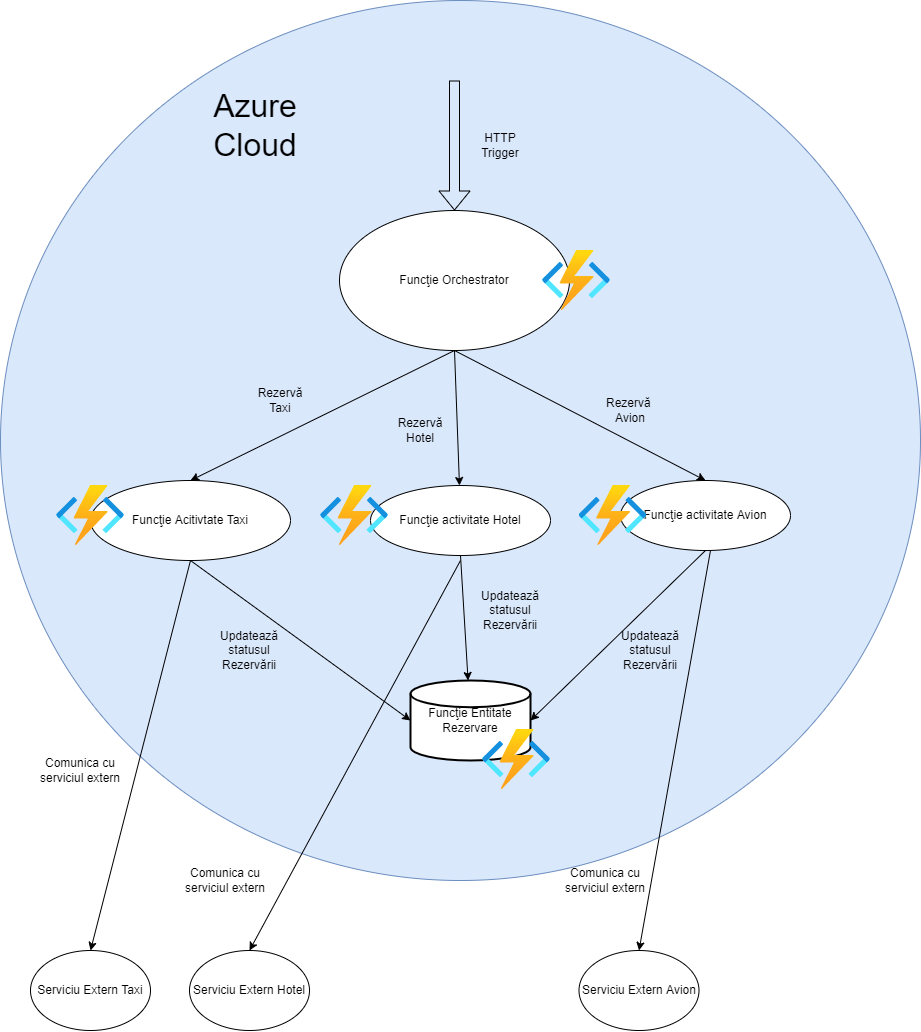
\includegraphics[width=1\textwidth]{images/durable_functions_arhitecture}
			 \caption{Rezervare distribuită folosind Durable Functions}
			 \label{fig:durable-functions-booking-arhitecture}
\end{figure}
 \par Analizând ~\ref{fig:durable-functions-booking-arhitecture} putem observa următoarea corespondenţă între conceptele de bază expuse de Durable Functions, şi necesităţile noastre : 
 \begin{itemize}
 \item Nucleul serviciului nostru de gestiune al operaţiunii de rezervare este plasat într-o funcţie de orchestrare, ce garantează execuţia durabilă a logicii, astfel încât Saga să fie executată cu succes indiferent de eventualele întreruperi mecanice sau excepţii neaşteptate în timpul execuţiei.
 \item Fiecare interacţiune cu serviciile externe este izolată într-o funcţie de activitate, pentru a permite execuţia lor conform unor politici de retry şi pentru a izola comportamentul nedeterminist (apeluri asincrone prin reţea) de logica principală de orchestrare.
 \item Starea generală a rezervării este stocată prin intermediul unei funcţii entitate ce asigură capacitatea de a citi şi updata starea rezervării în mod distribuit, pe măsura ce serviciile externe procesează request-urile trimise de către serviciul principal.
 \end{itemize}
 \par Analizând strict codul de orchestrare putem observa că acesta nu este cu mult mai complex, doarece conceptele de durabilitate sunt abstractizate sub interfeţe uşor de folosit. 
\begin{lstlisting}[numbers=left]
var entityGuid = context.GetInput<string>();
var entityId = new EntityId(nameof(Booking), entityGuid);
var booking = await context.CallEntityAsync<Booking>(entityId, "Get");
var isHotelBooked= await context.CallActivityAsync<bool>("BookHotel", null);
booking = await context.CallEntityAsync(new EntityId(nameof(Booking), entityGuid),"UpdateHotel", isHotelBooked);
if (booking.Hotel)
  {
     var isTaxiBooked = await context.CallActivityAsync<bool>("BookTaxi", null);
     booking = await context.CallEntityAsync(new EntityId(nameof(Booking), entityGuid),"UpdateTaxi", isTaxiBooked);
     if (booking.Taxi)
       {
         var isFlightBooked = await context.CallActivityAsync<bool>("BookFlight", null);
         booking = await context.CallEntityAsync(new EntityId(nameof(Booking), entityGuid),"UpdateFlight", isFlightBooked);
       }
       else // hotel booked, taxi not booked - cancel hotel
       {
         await context.CallActivityAsync<bool>("CancelHotel", null);
         booking =  await context.CallEntityAsync(new EntityId(nameof(Booking), entityGuid),"UpdateHotel", false);
       }
       // hotel booked, taxi booked, flight not booked - cancel hotel & taxi
       if (booking.Hotel && booking.Taxi && !booking.Flight)
         {
           await context.CallActivityAsync<bool>("CancelHotel", null);
           booking = await context.CallEntityAsync(new EntityId(nameof(Booking), entityGuid),"UpdateHotel", false);
           await context.CallActivityAsync<bool>("CancelTaxi", null);
           booking = await context.CallEntityAsync(new EntityId(nameof(Booking), entityGuid),	"UpdateTaxi", false);
         }
   }
\end{lstlisting}
\par Folosind Durable Functions, codul de orchestrare se simplifică considerabil, deoarece excepţiile ce apar în cadrul unei orchestrări declanşează în mod automat marcarea acelei orchestrări ca fiind \emph{Failed}, ceea ce poate fi monitorizat în mod automat pentru a fixa eventualele cazuri de eşec pe flow-ul de rollback. 
\par Din punct de vedere al structurii codului, acesta descrie în mod procedural maşina de stări ce este implementată de serviciu, iar framework-ul asigură execuţia acestuia în mod durabil, printr-un mecanism de execuţie al orchestrării bazat pe event-sourcing. Practic, orchestrarea este re-executată de fiecare data când un eveniment este înregistrat pentru aceasta. Evenimentele pot avea diferite surse, interne sau externe. Evenimentele externe sunt cele iniţiate de utilizatori sau alte servicii, de exemplu cand serviciul de orchestrare este anunţat printr-un eveniment că o anumită acţiune s-a terminat. Evenimentele interne sunt cele care determină re-execuţia unei orchestrări când un cronometru durabil care ii se adresează expiră, sau o sub-orchestrare sau o activitate ce este înlănţuită în mod direct este finalizată. 
\par Atunci când o orchestrare este re-executată, aceasta sare în mod automat peste paşii care au fost executaţi deja. De fiecare dată cand prin intermediul contextului este inregistrată o sub-acţiune a unei orchestrări, o intrare în tabela de istoric este generată care inregistrează statusul şi eventualul rezultat al acelei sub-acţiuni. Atunci când orchestrarea este re-executată, aceasta încarcă din baza de date toţi paşii care au fost deja executaţi şi înregistrează doar acţiunile noi ce trebuiesc înregistrate. Astfel, este practic suportată în mod standard o strategie care minimizează request-urile către serviciile terţe şi care oferă o garanţie de execuţie cel putin o dată a activităţilor, fără însă a abuza în mod activ de aceasta. În cazul în care pe perioada execuţiei nici o exceptie neaşteptată nu apare, fiecare activitate este executată exact o dată. Acest suport care în mod clasic necesită destul de mult design şi efort de implementare este oferit de către Durable Functions, acesta fiind un alt avantaj pentru a alege această tehnologie pentru a manageria workflow-uri de lungă durată în cloud. 
\par La nivelul Activităţilor, acestea gestionează comunicarea cu serviciile externe. Din punct de vedere al execuţiei acestea sunt rulate urmând o garanţie de cel puţin o dată, iar din acest motiv implementarea lor este necesar să fie idempotentă, pentru a evita potenţialele acţiuni duplicate, în cazul unei execuţii multiple. Pe de altă parte, din cauză ca acestea nu sunt re-executate de mai multe ori în mod recurent, acestea nu trebuie să respecte aceleaşi restricţii ca orchestrările, şi pot avea comportament nedeterminist. Rezultatul acestora este returnat către orchestrări, iar acestea la rândul lor updatează entitatea care menţine starea rezervării. 
\subsection{Cronometre Durabile în Durable Functions}
\quad Cronometrele Durabile sunt suportate în mod standard de către Durable Functions prin intermediul contextului de execuţie. Conceptul din spate e asemănător cu cel propus în capitolul anterior, dar diferă deoarece cronometrul odată înregistrat, este gestionat ca un eveniment de sine stătător, şi nu este strâns legat de execuţia orchestrării. 
\begin{lstlisting}[numbers=left]
DateTime expireAt = context.CurrentUtcDateTime.AddHours(48);
var cts = new CancellationTokenSource()
var timeoutTask = context.CreateTimer(expireAt, cts);
if (!booking.isHotelBooked){
	var hotelBookingTask = context.CallActivityAsync<bool>("BookFlight", null);
	Task winner = await Task.WhenAny(hotelBookingTask, timeoutTask);
    if (winner == hotelBookingTask)
    {
    	cts.Cancel();
       booking = await context.CallEntityAsync(new EntityId(nameof(Booking), entityGuid),"UpdateFlight", isFlightBooked);
    }
    else
    {
       throw new TimeoutException(''The Timer expired before receiving a response from the hotel activity'');
    }
	}	
}
\end{lstlisting}
\par Putem observa că timpul mereu este calculat folosind timpul curent extras din contextul de execuţie. Acesta este un mod determinist de a extrage timpul curent, fiindcă va returna mereu aceeaşi valoare, chiar dacă orchestrarea este re-executată la diverse momente în timp. După crearea iniţială, acest timer este înregistrat în baza de date, iar în momentul în care acesta expiră, va declanşa o re-execuţie a orchestrării. În acel moment timer-ul va fi fost finalizat şi, urmărind codul de mai sus, se va arunca o excepţie. Dacă până în momentul în care timer-ul expiră este finalizată altă acţiune care concura cu timer-ul, atunci timer-ul trebuie să fie explicit închis folosind CancellationToken-ul pentru a preveni re-execuţii inutile ale orchestrării. În cazul in care timer-ele rămân deschise chiar şi atunci când nu mai sunt aşteptate, acest lucru duce la o degradare a performanţei funcţiilor noastre durabile. 
\subsection{Considerente de deployment şi scalabilitate}
\quad Din punct de vedere al deployment-ului soluţia ce foloseşte Durable Functions suferă de ''vendor lock-in''. Acest lucru înseamnă că soluţia aceasta nu este generică din punct de vedere al deployment-ului, şi dezvoltatorul are o singură soluţie: deployment-ul în Azure Cloud folosind Durable Functions. Execuţia soluţiei on-prem sau portarea acesteia către un alt provider de soluţii cloud nu este posibilă. 
\par În schimb, soluţia disponibilă de a rula aplicaţia folosind Durable Functions, vine cu 2 mari avantaje : 
\begin{itemize}
\item Scalare pe orizontală infinită, fără restricţii de performanţă şi fără complexitate suplimentară în nivelul de rutare, deoarece acest lucru este deja gestionat de Azure.
\item Mod de calcul al costurilor foarte avantajos, deoarece se plăteşte doar timpul de execuţie, nu şi timpul de aşteptare. Iar într-un sistem în care timpul de execuţie reprezintă mai puţin de 2\% din timpul total de viaţă a workflow-ului (deoarece majoritatea timpului este petrecut asteptând timere sau evenimente externe) acest lucru este foarte valoros şi duce la o reducere considerabilă a costurilor de execuţie a unui astfel de sistem. 
\end{itemize}
\par Deşi această limitare a opţiunilor de deployment poate fi o vulnerabilitate pe viitor, pentru moment această soluţie este cea mai bună deoarece în piaţă nu există un competitor care să ofere tehnologie stateful serverless într-un mod mai bun.  
\subsection{Arhitectura non-serverless pentru execuţia durabilă a workflow-urilor}
\quad Arhitectura serverless vine cu numeroase beneficii, mai ales în zona de management a deploymentului şi a scalabilităţii automate. În schimb, aşa cum a fost punctat şi in secţiunea anterioară, alegerea acestei modalităţi de execuţie suferă de ''vendor lock-in'', iar acest lucru poate fi un impediment pentru anumite companii, care preferă flexibilitate pe termen lung. 
\par Alternativa la a lansa serviciul de management a workflow-urilor ca funcţii serverless durabile, este să fie folosit framework-ul ce stă la baza acestora (Durable Task Framework), într-un mod self-hosted. Acest lucru inseamnă că din punct de vedere al infrastructurii, aplicaţia va semăna cu varianta iniţială analizată, care nu folosea nici un framework. Serviciul va rula pe un server web clasic, având ca suport la nivelul stocării datelor, o bază de date relaţională (aici DTF oferă mai multe opţiuni, dar pentru exemplul curent vom analiza varianta în care DTF providerul este bazat pe SQLServer).
Din punct de vedere al scalabilităţii, această configuraţie are aceleaşi avantaje şi dezavantaje ca orice aplicaţie web clasică. În schimb, din punct de vedere al managementului de workflow-uri de lungă durata, folosind DTF, toate primitivele necesare sunt deja implementate reducând semnificativ timpul de dezvoltare al unui astfel de serviciu. Astfel, putem pune DTF în categoria serviciilor ce îmbunătaţesc productivitatea dezvoltatorilor.
 \begin{figure}[h]
\centering
        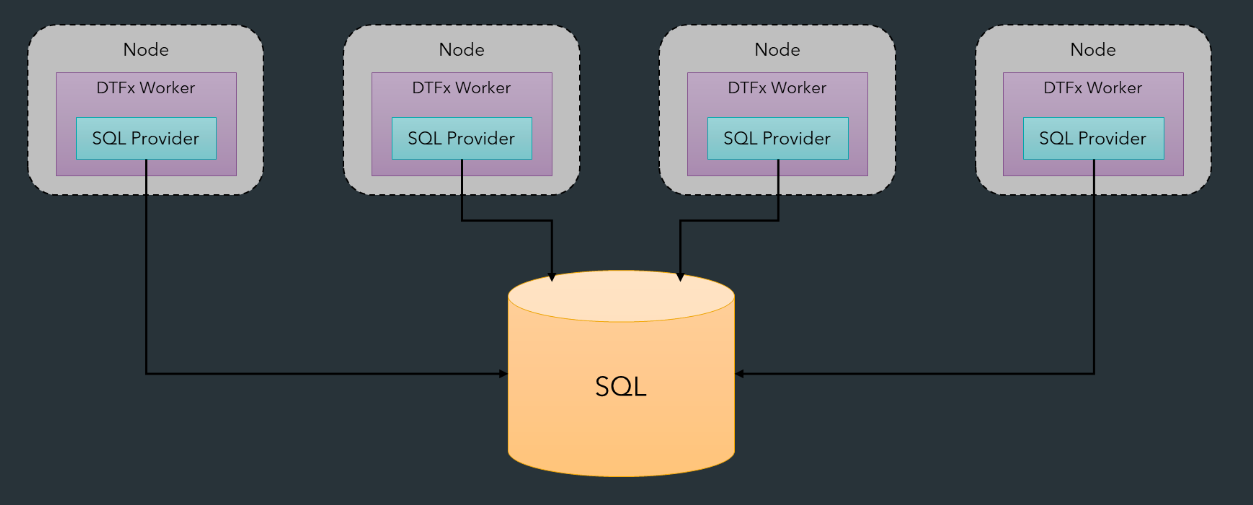
\includegraphics[width=1\textwidth]{images/dtf_scaling}
			 \caption{Scalare automată a workerilor DTF}
			 \label{fig:dtf-scaling}
			 \source {https://microsoft.github.io/durabletask-mssql}
\end{figure}
\par Aşa cum se poate observa şi în figura ~\ref{fig:dtf-scaling}, DTF realizează acelaşi potenţial de scalabilitate ca sistemul clasic analizat iniţial, prin posibilitatea de a adauga mai mulţi workeri (instanţe ale serviciuliu ce foloşeste DTF) conecţaţi la aceeaşi bază de date. Acest lucru este posibil, printr-un mecanism de locking la nivelul bazei de date, ce previne mai mulţi workeri să consume aceeaşi muncă în mod concurent. Fiecare worker execută un mecanism de polling la nivelul bazei de date, ce încearcă să rezerve un work-item pentru acesta. Atât timp cât logica de selecţie a următorului work-item este rezistentă la execuţii paralele, atunci un numar nelimitat de workeri pot fi adaugaţi împotriva unei baze de date. 
\par Abilitatea de a scala orizontal numărul de workeri conectaţi la o bază de date, evidenţiază în acelaşi timp şi vulnerabilitatea acestui sistem: Baza de date poate limita performanţa sistemului, dacă numărul de workeri conectaţi la aceasta este prea mare. Singura soluţie pentru a îmbunătăţi performanţa sistemului atunci când limitele bazei de date sunt atinse, este scalarea pe verticală a acesteia. Însa, scalarea pe verticală nu poate fi infinită, din cauza limitărilor din punct de vedere hardware care există acum în industrie. 
\par Pentru a scala pe orizontală şi la nivelul bazei de date, trebuie implementat un mecanism de sharding, ce conţine şi logică de rutare, asemănător celui descris în secţiunile anterioare. Acest lucru este necesar pentru a garanta că evenimentele transmise către un anume workflow ajung către instanţa care a şi creat acel workflow. 
\chapter {Rezultate şi concluzii}
\quad Rezolvarea unei probleme comune a fost abordată în două moduri diferite. În urma acestui efort, au fost identificate numeroase probleme generice de care dezvoltatorii se lovesc atunci când doresc să dezvolte sisteme durabile, ce pot orchestra workflow-uri de lungă durată, într-un sistem distribuit. 
\par Dezvoltarea unui sistem de management al workflow-urilor de lungă durată într-un mediu distribuit este o problemă cu foarte multe cazuri speciale, mai ales în zona durabilităţii sistemului şi garanţiilor de execuţie pe care acesta le oferă. 
\par Observând caracterul repetabil al acestor cazuri speciale, în piaţă au aparut diverse framework-uri care rezolvă în mod generic aceste probleme şi expun interfeţe uşor de consumat, printre care cel mai matur fiind DurableTaskFramework. Folosind această tehnologie, a fost dezvoltat un serviciu demonstrativ, ce rezolvă problema rezervării unei excursii şi care expune o metodă interactivă de a vizualiza managementul unei tranzacţii distribuite. Aplicaţia este accesibilă în mod public la \emph{https://durable-saga-front-end.web.app/}. 
\par Primitivele expuse de Durable Functions au înjumătăţit timpul de dezvoltare a soluţiei şi au generat un serviciu cu costuri aproape de 0, deoarece sistemul este în totalite serverless. 
\par Pe viitor vor fi abordate eventuale îmbunătăţiri ale DTF în zonele în care au fost descoperite vulnerabilităţi în cadrul acestei lucrări, respectiv în adăugarea suportului pentru throttling în DTF.
\listoffigures
\addcontentsline{toc}{section}{Bibliografie}
\bibliographystyle{abbrv}
\bibliography{\jobname}
\end{document}